\documentclass{beamer}

\mode<presentation>
{
  \usetheme{Madrid}
  \setbeamertemplate{navigation symbols}[horizontal]
  \setbeamertemplate{caption}[numbered]
  \usecolortheme{seahorse}
}

\usepackage[utf8]{inputenc}
\usepackage[T1]{fontenc}
\usepackage[french]{babel}
\usepackage{booktabs}
\usepackage{tabularx}
\usepackage{fontawesome5}
\usepackage{listings}
\usepackage{xcolor}
\usepackage{tikz}
\usepackage{float}
\usetikzlibrary{shapes.geometric, arrows.meta, positioning, calc, shadows.blur}

% --- Configuration du style de code ---
\definecolor{codebg}{rgb}{0.98,0.98,0.98}
\definecolor{codegray}{rgb}{0.5,0.5,0.5}

\lstset{
    backgroundcolor=\color{codebg},
    basicstyle=\ttfamily\scriptsize,
    breaklines=true,
    numbers=left,
    numberstyle=\tiny\color{codegray},
    stepnumber=1,
    numbersep=8pt,
    frame=single,
    rulecolor=\color{black!20},
    captionpos=b,
    xleftmargin=2em,
    framexleftmargin=1.5em
}

% --- Nettoyage du Titre et Auteurs (Fix hyperref warnings) ---
\title[Nom du module]{Nom du module \\ Titre de la présentation}

\author[P. Nom \& P. Nom]{
    \textbf{Présenté par :}\\
    Prénom NOM \& Prénom NOM 
    \texorpdfstring{\\ \medskip}{ } 
    \textbf{Encadré par :}\\
    Pr. Prénom NOM
}

\institute{Projet académique – Module Nom du module}
\date{\today}

\begin{document}

\begin{frame}
  \begin{center}
    
\includegraphics[width=0.3\linewidth]{logos/logo_FSR.jpg}
  \end{center}
  \vspace{-0.6cm}
  \titlepage
\end{frame}

\begin{frame}[plain]
    \tableofcontents
\end{frame}

\section{Introduction}
\begin{frame}{Introduction}
\begin{block}{Contexte}
Présentez le contexte du projet en deux ou trois phrases.
Mettez en avant les \textbf{mots-clés} importants.
\end{block}
\end{frame}

\begin{frame}
\centering
{ \Huge la Problématique}
\end{frame}

\begin{frame}{Problématique du projet}
\begin{block}{Problème ciblé}
\begin{itemize}
\item Problème 1
\item Problème 2
\item Problème 3
\end{itemize}
\end{block}

\begin{block}{Objectif de notre projet}
Développer une solution capable de :
\begin{itemize}
\item Objectif 1
\item Objectif 2
\item Objectif 3
\end{itemize}
\end{block}
\end{frame}

\begin{frame}
\centering
{ \Huge Les notions de bases}
\end{frame}

\section{Notions Fondamentales du Projet}
\begin{frame}{Notions abordées dans ce projet}
\begin{block}{Technologies clés}
\begin{itemize}
\item Notion 1
\item Notion 2
\item Notion 3
\end{itemize}
\end{block}
\end{frame}

\begin{frame}{Notion 1}
\begin{block}{Définition}
Définition de la notion.
\end{block}
\begin{block}{Caractéristiques}
\begin{itemize}
\item Caractéristique 1
\item Caractéristique 2
\item Caractéristique 3
\end{itemize}
\end{block}
\end{frame}

\begin{frame}{Notion 2}
\begin{block}{Rôle}
Rôle de cet élément dans le projet.
\end{block}
\begin{table}
\centering
\begin{tabular}{ll}
\toprule
Élément & Rôle \\
\midrule
Élément 1 & Rôle \\
Élément 2 & Rôle \\
Élément 3 & Rôle \\
\bottomrule
\end{tabular}
\end{table}
\begin{figure}
    \centering
    
\includegraphics[width=0.2\linewidth]{logo.png}
    \caption{Logo}
\end{figure}
\end{frame}

\begin{frame}
\begin{figure}
    \centering
    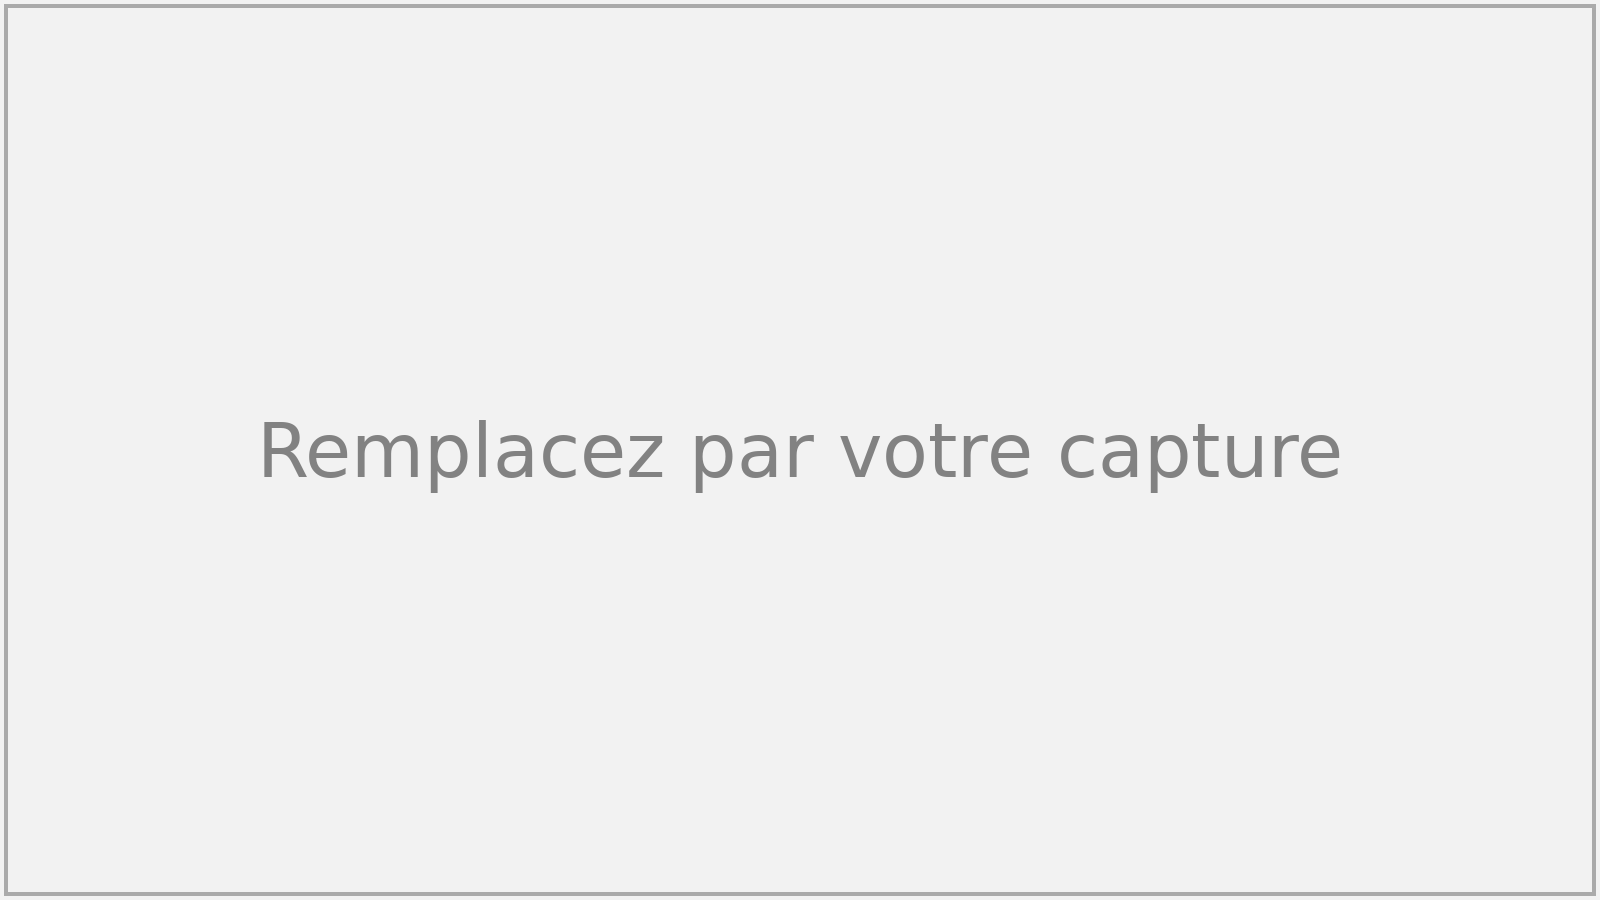
\includegraphics[width=0.8\linewidth]{capture.png}
    \caption{Titre de la figure}
\end{figure}
\end{frame}

\section{Architecture du Projet}
\begin{frame}{Architecture globale}
\begin{figure}[H]
    \centering
    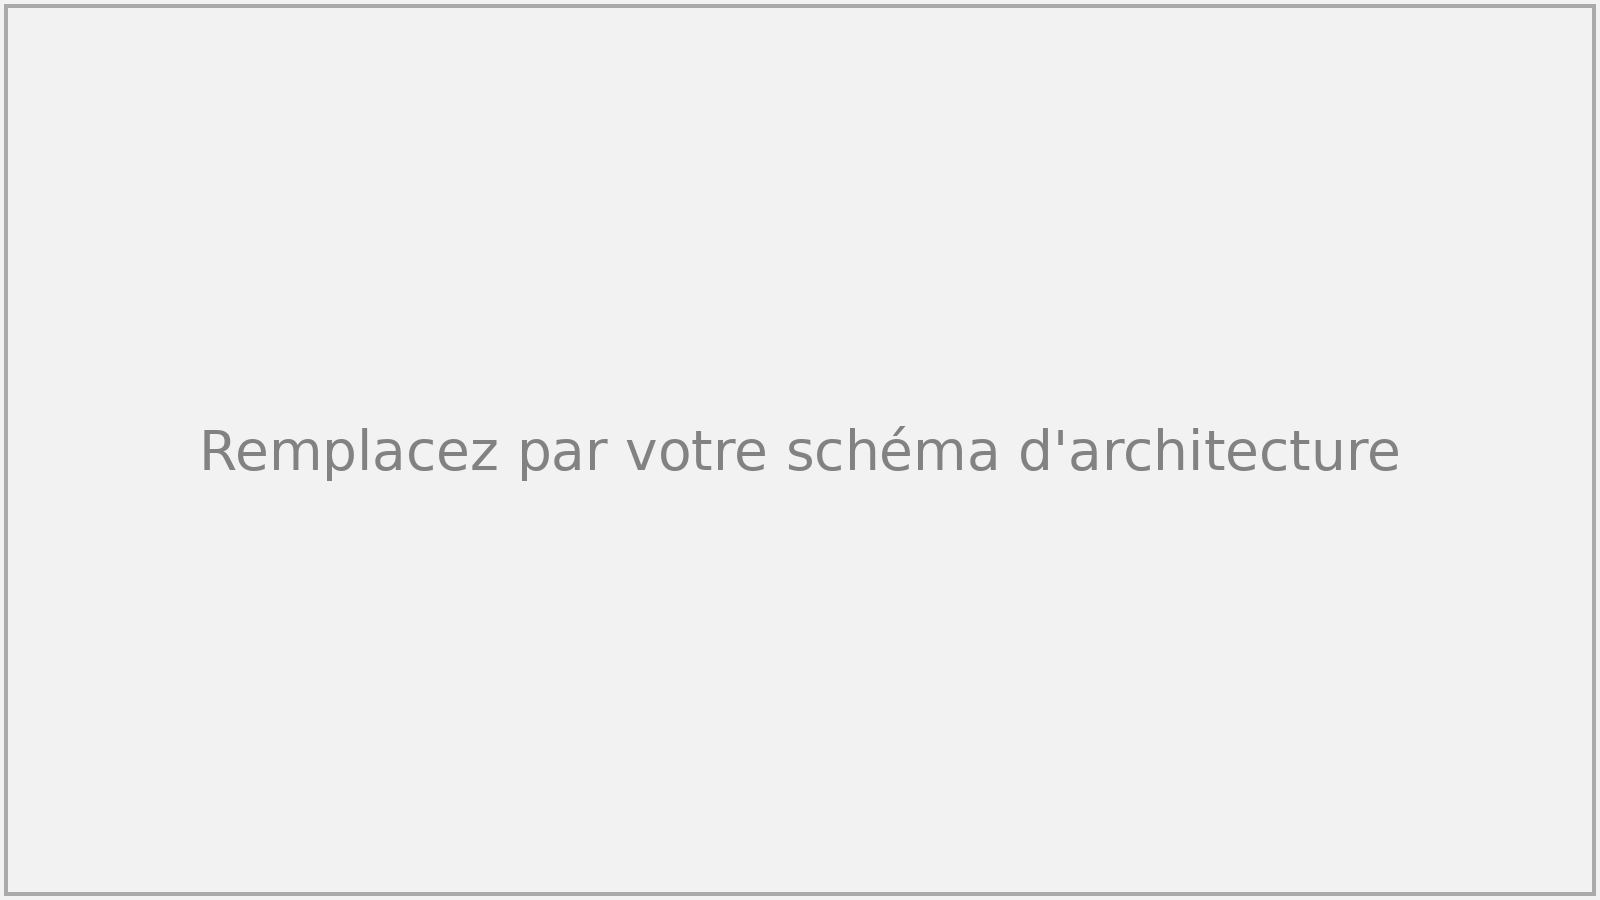
\includegraphics[width=0.8\linewidth]{architecture.png}
    \caption{Architecture}
\end{figure}
\end{frame}

\begin{frame}{Choix techniques}
\begin{block}{Choix technique}
Justifiez le choix principal.
\end{block}
\end{frame}

\section{Réalisation}
\begin{frame}{Étapes de réalisation}
\begin{block}{Étapes}
    \begin{itemize}
    \item \textbf{Étape 1} : Description.
    \item \textbf{Étape 2} : Description.
    \item \textbf{Étape 3} : Description.
\end{itemize}
\end{block}
\end{frame}

\begin{frame}[fragile]{Exemple de code}
\begin{block}{Extrait}
\begin{verbatim}
commande --option argument
\end{verbatim}
\end{block}
\end{frame}

\section{Tests et Validation}
\begin{frame}{Tests}
\begin{block}{Objectif}
Décrivez le test réalisé et le résultat obtenu.
\end{block}
\end{frame}

\section{Conclusion}
\begin{frame}{Conclusion}
\begin{block}{Bilan}
Résumez le bilan du projet.
\end{block}
\begin{block}{Perspectives}
Présentez les perspectives.
\end{block}
\end{frame}

\begin{frame}
\centering
{ \Huge Merci pour votre attention}
\end{frame}

\end{document}
